\chapter{Progettazione}

\section{Progettazione MDSP}

\subsection{Protocollo di trasporto}
Considerando i requisiti, è stato scelto UDP come protocollo per il trasporto
dei messaggi.

\subsection{Messaggi}


Le componenti del sistema che si trovano su elaboratori differenti comunicano tra
loro per mezzo di 'messaggi'. Tali messaggi rappresentano una particolare
richiesta di servizi, oppure una corrispondente risposta.

Un messaggio possiede una 'tipologia' e un certo numero di 'argomenti', dipendenti dal tipo di messaggio.

Il tipico messaggio è composto da un header di 8 byte, cosi' suddivisi:



\begin{itemize}
\item 3 byte per la stringa MDC

\item 1 byte per la versione del protocollo

\item 4 byte per il tipo di messaggio
\end{itemize}

I messaggi possono avere una o più stringhe ``null-terminated'',
ognuna delle quali descrive uno o più parametri. I parametri hanno un
\emph{nome} e un \emph{valore}, e più parametri sono separati dal segno di
``;'' (punto e virgola). L'esempio seguente:

\begin{code}
n=nome;h=12;
\end{code}

mostra due parametri: \emph{n} che ha valore ``\emph{nome}'' e \emph{h} con
valore \emph{12}.

Vedremo nelle sezione seguenti i principali messaggi e i loro parametri.




\subsubsection*{LIST}
%
\emph{LIST} è un messaggio utilizzato quando di vuole conoscere la lista degli
stream multimediali presenti su un certo host.

Parametri:
\begin{itemize}
  \item \emph{n}: stringa che indica il nome o un suo frammento, usata per
  circoscrivere la ricerca
\end{itemize}

\subsubsection*{ALST}
%
\emph{ALST} (contrazione di ``Answer LiST'') è la tipica risposta ad un
messaggio LIST. Il primo byte del contenuto rappresenta il numero di stream
trovati, ed è seguito da stringhe null-terminated contenenti i seguenti
parametri:
\begin{itemize}
  \item \emph{n}: stringa con il nome completo dello stream
  \item \emph{h}: stringa di 32 byte che rappresenta lo \emph{stream id}
  (univoco per tutto il sistema)
\end{itemize}

\subsubsection*{SINF}
\emph{SINF} (contrazione di ``Stream INFormation'') è usato per richiedere
informazioni su un determinato stream multimediale, come il numero di
descrizioni in cui è suddiviso e il numero di descrittori.

Parametro:
\begin{itemize}
  \item \emph{h}: \emph{stream id} dello stream richiesto
\end{itemize}

\subsubsection*{ASNF}
%
\emph{ASNF} (contrazione di ``Answer Stream iNFormation'') è generato in
risposta ad un messaggio SINF.

Parametri:
\begin{itemize}
  \item \emph{h}: \emph{stream id} dello stream multimediale richiesto
  \item \emph{fn}: \emph{flows numebr}, ossia il numero totale di
  \emph{descrizioni} (sotto-flussi MDC)
  \item \emph{sn}: \emph{sequence number}, ossia il numero totale di descrittori
\end{itemize}


\subsubsection*{SREQ}
%
\emph{SREQ} (contrazione di ``Stream REQuest'') viene utilizzato per richiedere
determinati descrittori di un particolare stream.

Parametri:
\begin{itemize}
  \item \emph{h}: \emph{stream id} dello stream multimediale richiesto
  \item \emph{f}: \emph{flow id}, ossia identificativo della particolare
  \emph{descrizione} (sotto-flusso)
  \item \emph{sb}: \emph{sequence begin}, ossia il numero del primo descrittore
  della sequenza richiesta
  \item \emph{se}: \emph{sequence end}, ossia il numero dell'ultimo descrittore
  della sequenza richiesta
\end{itemize}


\subsubsection*{ASRQ}
%
\emph{ASRQ} (contrazione di ``Answer Stream ReQuest'') viene utilizzato in
risposta al messaggio SREQ, come conferma dell'inizio dell'invio dei
descrittori scelti. 

Parametri:
\begin{itemize}
  \item \emph{h}: \emph{stream id} dello stream multimediale richiesto
  \item \emph{f}: \emph{flow id}, ossia identificativo della particolare
  \emph{descrizione} (sotto-flusso)
  \item \emph{sb}: \emph{sequence begin}, ossia il numero del primo descrittore
  della sequenza richiesta
  \item \emph{se}: \emph{sequence end}, ossia il numero dell'ultimo descrittore
  della sequenza richiesta
\end{itemize}

Contiene gli stessi parametri di SREQ, ma i valori sono
modificati in relazione allo stato dell'host. Per esempio, se vengono chiesti i
descrittori in una sequenza da 0 a 30, mentre l'host dispone soltanto dei
descrittori da 4 a 10, allora ASRQ conterrà $sb=4$ e $se=10$.

Subito dopo l'invio di un messaggio ASRQ l'host inizierà ad inviare i
descrittori richiesti sul canale dati.



\subsection{Descrittore}


Un \emph{Descriptor} è, nell'ambito di questo sistema, una unità di dati di un
flusso multimediale.

Il flusso multimediale è suddiviso in sotto-flussi detti \emph{descrizioni},
secondo le specifiche della codifica MD; ogni descrizione è composta da un certo numero
di descrittori, con la stessa relazione che c'è tra un filmato e un fotogramma.

Il Descriptor contiene varie informazioni, come il flusso originario, il numero
di descrizione, e la sequenza temporale. Il payload non è definito e pertanto è
permessa una maggiore libertà in fase di definizione dei codec.

\subsection{Casi d'uso}

Chiameremo Alice un generico nodo della rete che vuole effettuare le azioni, e
Bob il peer a cui queste comunicazioni sono dirette.

Ci sono poi anche altri amici, come Carlina, David ed Emy, che condividono le
stesse passioni di Alice e Bob.


\subsubsection{Richiesta di un flusso multimediale}
%

Alice ha bisogno di un flusso multimediale, e sa già che Bob ce l'ha, tutto o in
parte (lo sa perché ha già visto la lista dei flussi di Bob).

Quindi Alice invia un messaggio SREQ, specificando come parametro l'hash univoco
del flusso, il numero della descrizione, e una sequenza di descrittori.

Bob quindi invierà un messaggio ASRQ, specificando come parametro il timeout di
keep-alive; Bob, infatti, continuerà ad inviare il flusso di dati finché riceverà
pacchetti di KALV (keep-alive) da Alice, supponendola disconnessa allo scadere
del timeout.






\subsubsection{Richiesta della lista dei flussi}
%

\begin{itemize}
\item Alice ha bisogno della lista dei flussi disponibili da Bob. Invia un messaggio LIST, non parametro vuoto, e riceve da Bob un messaggio ALST (Answer LiST) contenente un vettore con tutti i nomi e gli hash dei flussi che egli possiede;
\item Alice sta cercando un particolare flusso, di cui sa parte del nome
('pippo'); invia un messaggio LIST a Bob con parametro 'pippo', e Bob
risponderà con un ALST contenente informazioni su tutti i file che contengono la
parola 'pippo' nel nome.
\end{itemize}




\subsubsection{Richiesta di informazioni su un flusso}
%

Alice sa che un determinato flusso (di cui possiede l'hash) è posseduto da Bob;
invia quindi un messaggio SINF (Stream INFormation), per avere informazioni
specifiche del flusso, ad esempio la durata, la qualità di codifica, ecc. Bob
invia un messaggio ASNF contenente la risposta.






% \subsubsection{Invio di parametri di rete}
% %
% 
% Alice deve informare Bob di cambiamenti che stanno avvenendo dalla sua parte; per
% esempio, sta cambiando rete e non vuole interrompere lo streaming; oppure c'è
% stato un problema con il router ed è necessario abbassare la velocità di invio
% del flusso. In tutti questi casi, Alice invia un messaggio PARM a Bob,
% specificando i nuovi parametri.






% \subsubsection{Richiesta di altri peer con lo stesso flusso}
% %
% 
% Alice sta scaricando un flusso da Bob, ma avverte la necessità di frequentare
% altre persone, che magari condividono lo stesso flusso; invia quindi un messaggio
% PEER a Bob, seguito dall'hash univoco del flusso. Bob raccoglie le idee su tutti
% gli amici che conosce, o che ha conosciuto tramite lo scaricamento del flusso in
% oggetto, per esempio Carlina, da cui Bob ha scaricato originariamente il flusso,
% David, che ha scaricato il flusso tempo fa, ed Emy che lo sta scaricando ora. Bob
% quindi prepara un messaggio APER contenente l'indirizzo ip e la porta di Carlina,
% David ed Emy e lo invia ad Alice.







\section{Codec}
\label{cap:descrizione_codec}
Il paradigma di protocollo di streaming a descrittori multipli rende
necessaria la progettazione di codec su misura. Viene rimandata al capitolo
\ref{cap:implementazione_codec} la presentazione, a titolo esplicativo, del
\emph{codec testuale}.

\subsection{Caratteristiche del codec}
Affinché un codec possa funzionare con il protocollo MDC (\emph{Multiple
Description Coding}) è necessario che possieda delle caratteristiche ben
precise. La codifica MDC ha come obiettivo finale la descrizione di un file in
modo tale che, in caso di perdita parziale dei dati che lo costituiscono, il
file stesso sia ugualmente interpretabile. L'assoluta interpretabilità del
file costituisce un vincolo molto stringente e si rendono necessari codec
progettati con particolari accorgimenti. MDSP versione 0.1 gestisce file di
tipo testuale e immagini, consente di visualizzare il contenuto di un file anche
se si verificano errori nel trasferimento dello stesso attraverso una rete di telecomunicazione. Durante la fase di codifica il file sorgente viene suddiviso in descrizioni e descrittori:
\begin{itemize}
 \item Un descrittore è la più piccola unità di misura del contenuto di un
 file. L'insieme di più descrittori costituisce una descrizione.
 \item Una descrizione può contenere parte o tutte le informazioni di un file
 (con `informazioni' si intendono i dati costituenti il file).
\end{itemize}
Le descrizioni costituiscono differenti codifiche e devono essere il più possibile ortogonali fra loro, in modo da poter essere indipendenti l'una dall'altra, pur riferendosi tutte allo stesso file sorgente.

Nel caso in cui qualche descrizione venga persa, sia corrotta, o non venga
inviata dalla sorgente, sarà comunque possibile decodificare il file ed
otterene un output sufficientemente corretto, tale da poter essere intepretato. \`E sufficiente la ricezione di una sola descrizione per la corretta ricostruzione del file sorgente. La ricezione di due o più descrizioni migliora l'accuratezza del file decodificato. Il file sorgente viene `\emph{descritto}' con più precisione.  Tale risultato viene raggiunto grazie alla creazione di codec che tengono in considerazione il fattore umano nell'interpretazione di vari tipi di informazioni:
\begin{itemize}
 \item Nel caso del testo, una parola con una lettera mancante viene facilmente interpretata dal lettore. Il cervello umano sostituisce la lettera mancante con quella corretta basandosi sul senso della parola stessa o della frase.
 \item Nel caso delle immagini, la mancanza di pixel non rende l'immagine inutilizzabile. All'occhio umano saranno presenti delle lievi alterazioni, ma, anche questa volta, il contesto rende ugualmente interpretabile l'immagine e le informazioni che essa contiene.
\end{itemize}

\begin{figure}[ht]
\centering 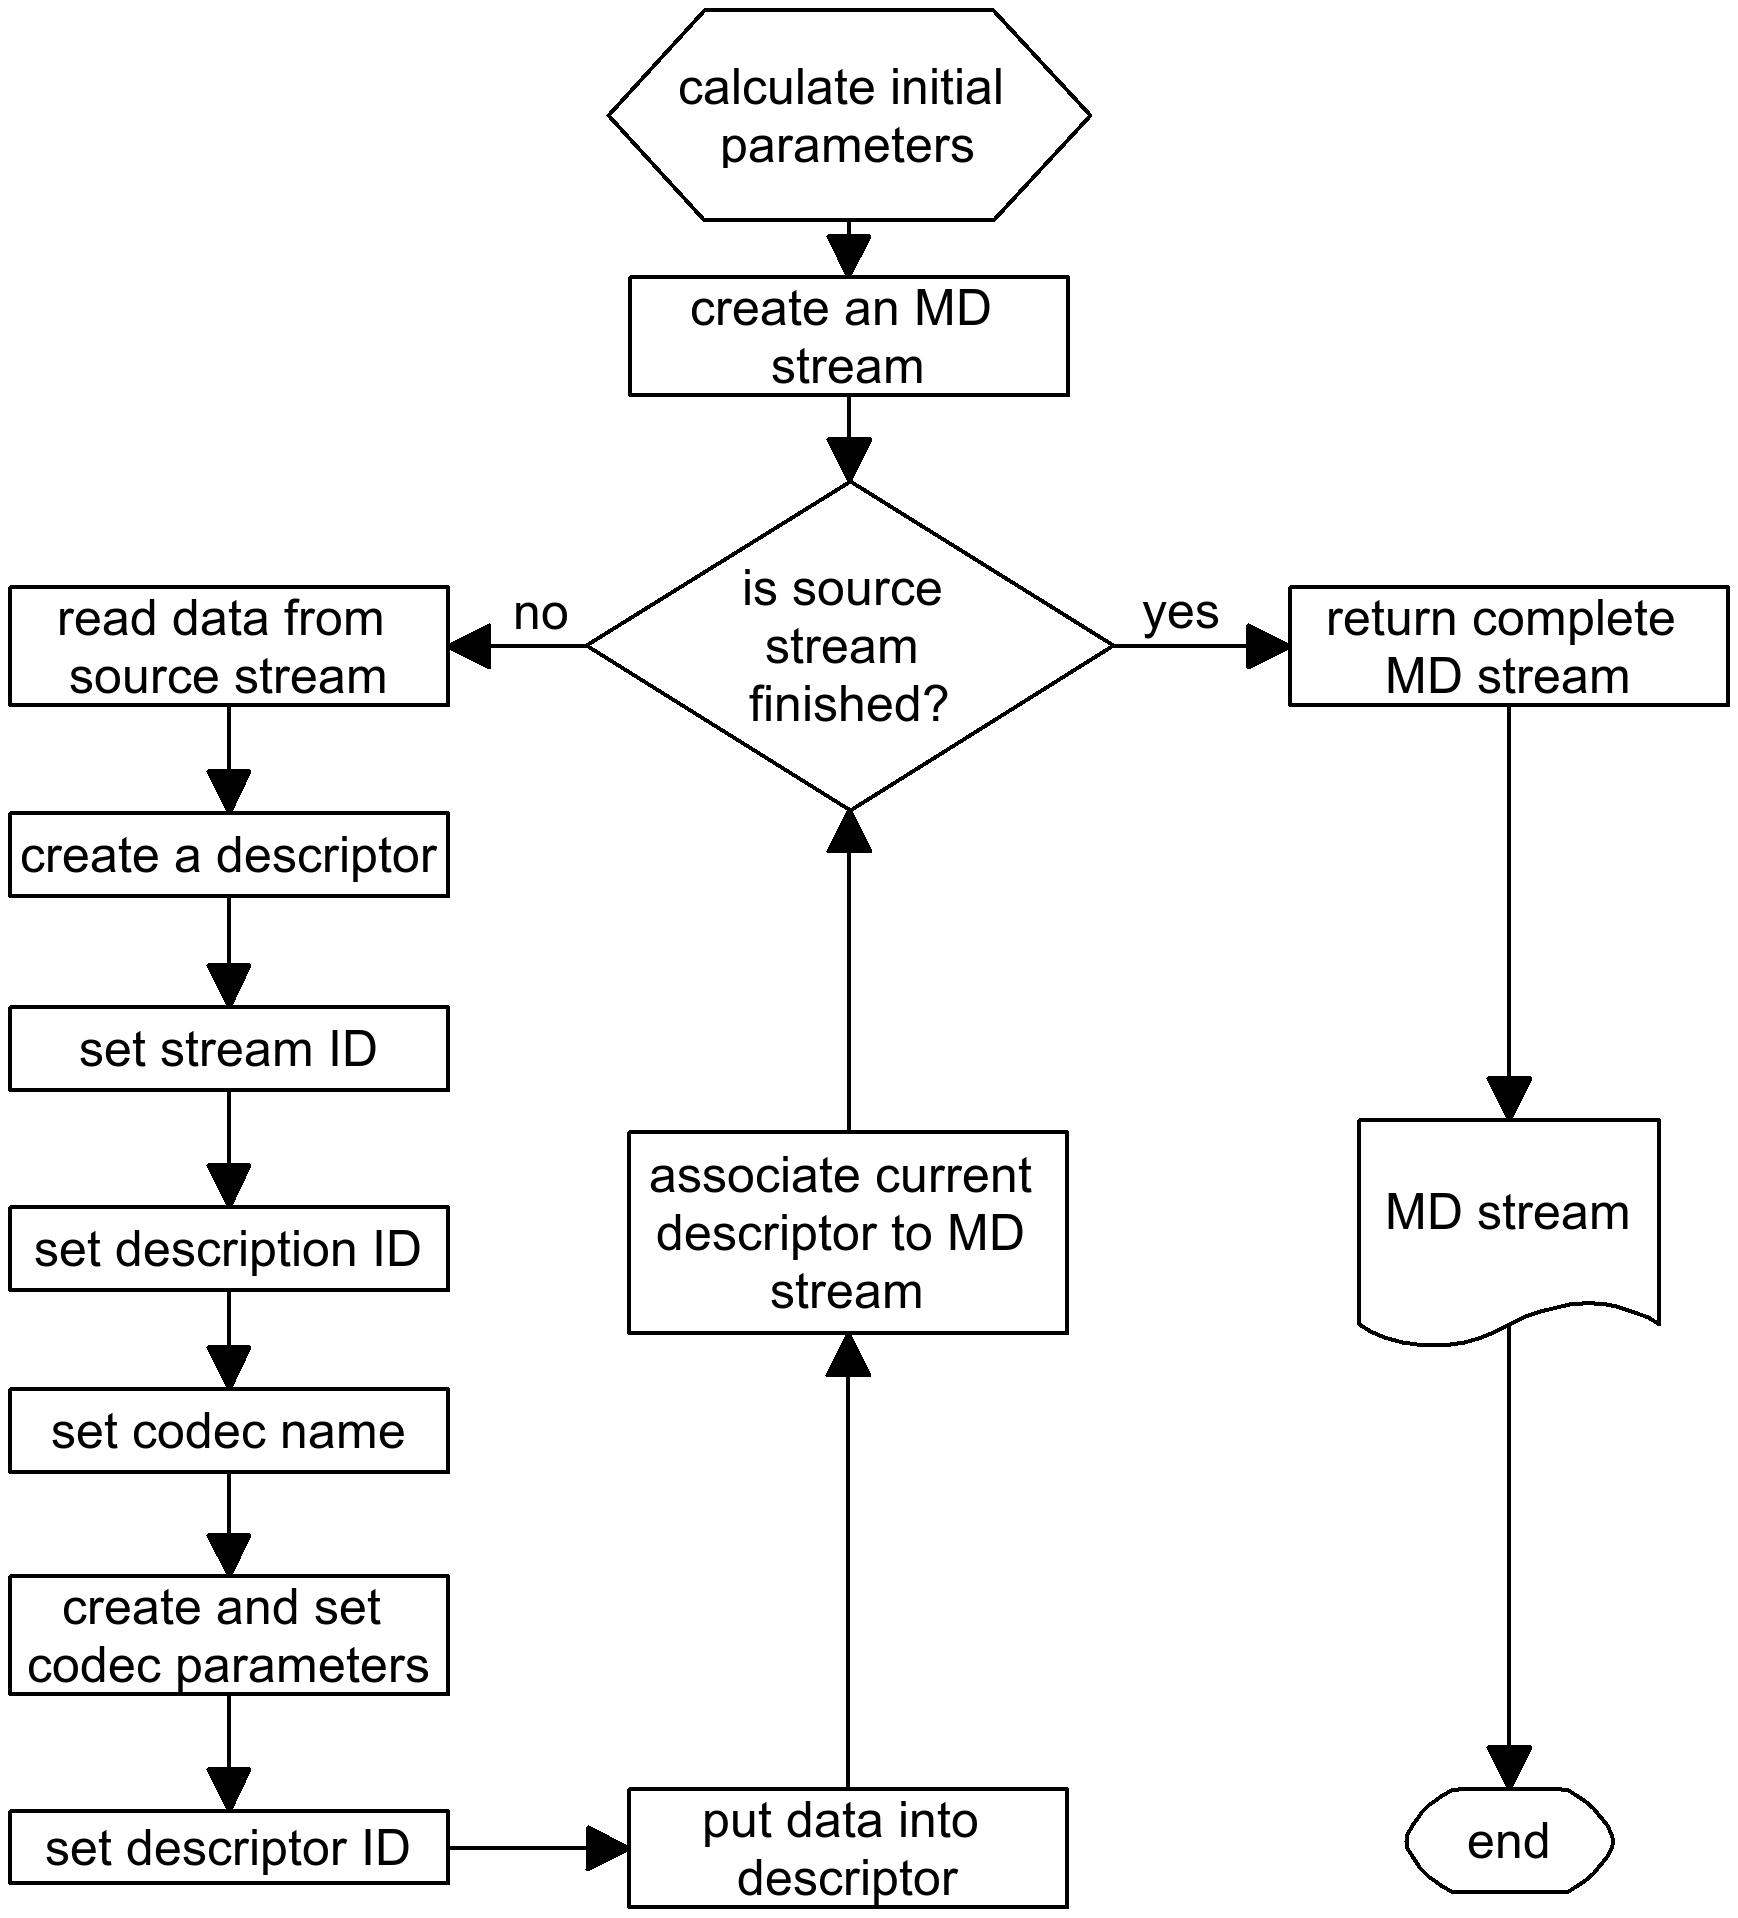
\includegraphics[width=0.90\textwidth]{../images/codifica.png}
	\caption{Diagramma di flusso dell'algoritmo di codifica.}
	\label{fig:codifica}
\end{figure}

\begin{figure}[ht]
\centering 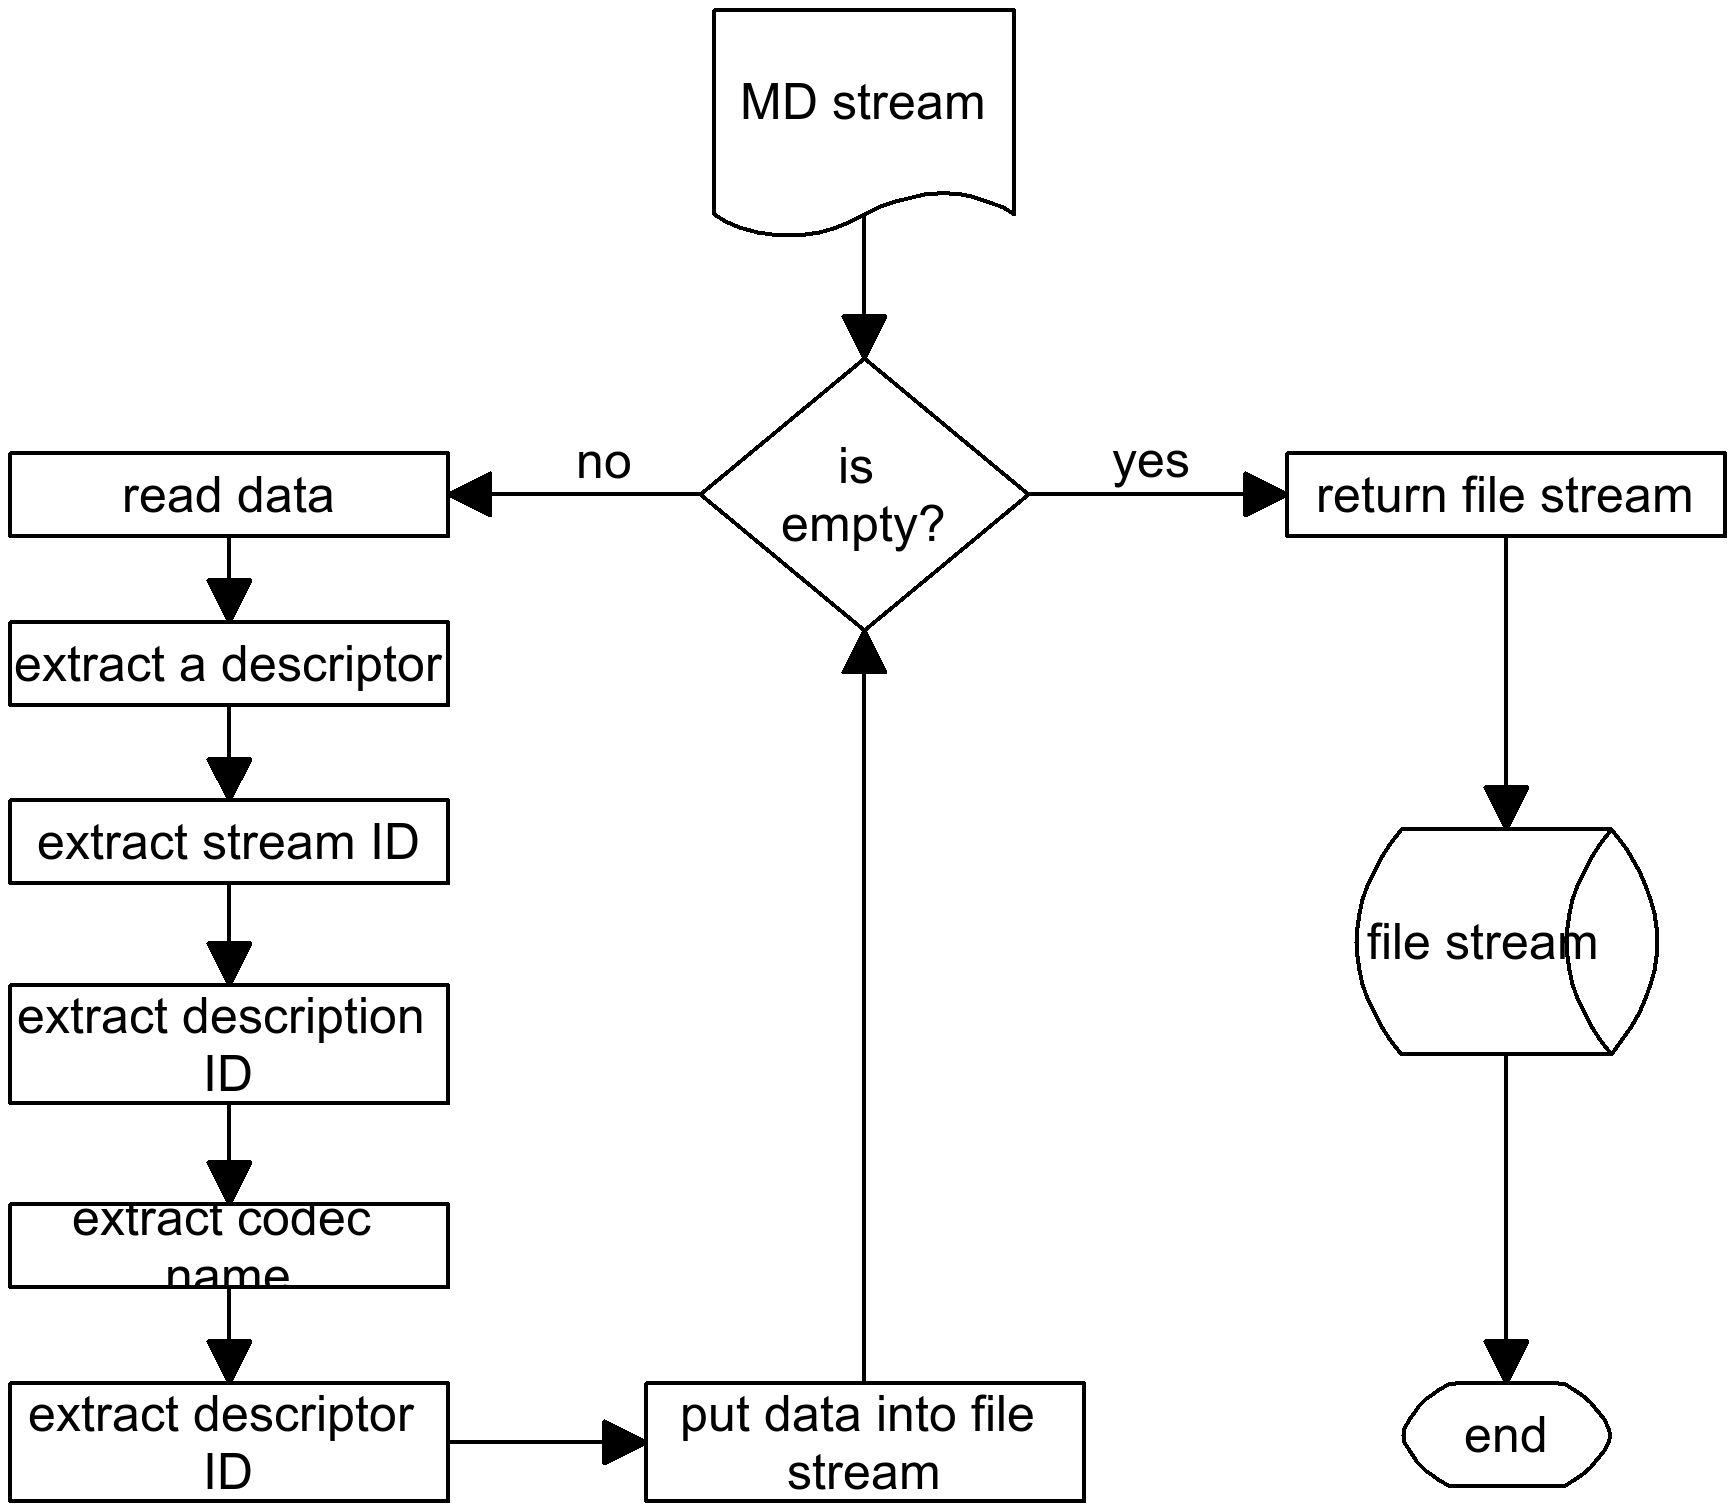
\includegraphics[width=0.90\textwidth]{../images/decodifica.png}
	\caption{Diagramma di flusso dell'algoritmo di decodifica.}
	\label{fig:decodifica}
\end{figure}

Il funzionamento del codec (illustrato in figura \ref{fig:codifica} e
\ref{fig:decodifica}) si può applicare per descrivere la suddivisione di ogni
descrizione in descrittori. Come accennato, i descrittori sono la più piccola unità di memorizzazione dei dati costituenti il file sorgente. Tale
affermazione significa che, se viene perso un descrittore durante il
trasferimento, oppure i suoi dati non sono corretti, esso può essere
semplicemente non considerato. Ciò permette un'estrema flessibilità di
decodifica. Sostanzialmente, il decodificatore deve adattarsi alla tipologia e
quantità di dati collezionati e creare un file di output. Tale file sarà perfetto se non si sono verificate perdite, o ugualmente interpretabile in presenza di perdite.
